% Created by tikzDevice version 0.11 on 2018-08-15 18:48:50
% !TEX encoding = UTF-8 Unicode
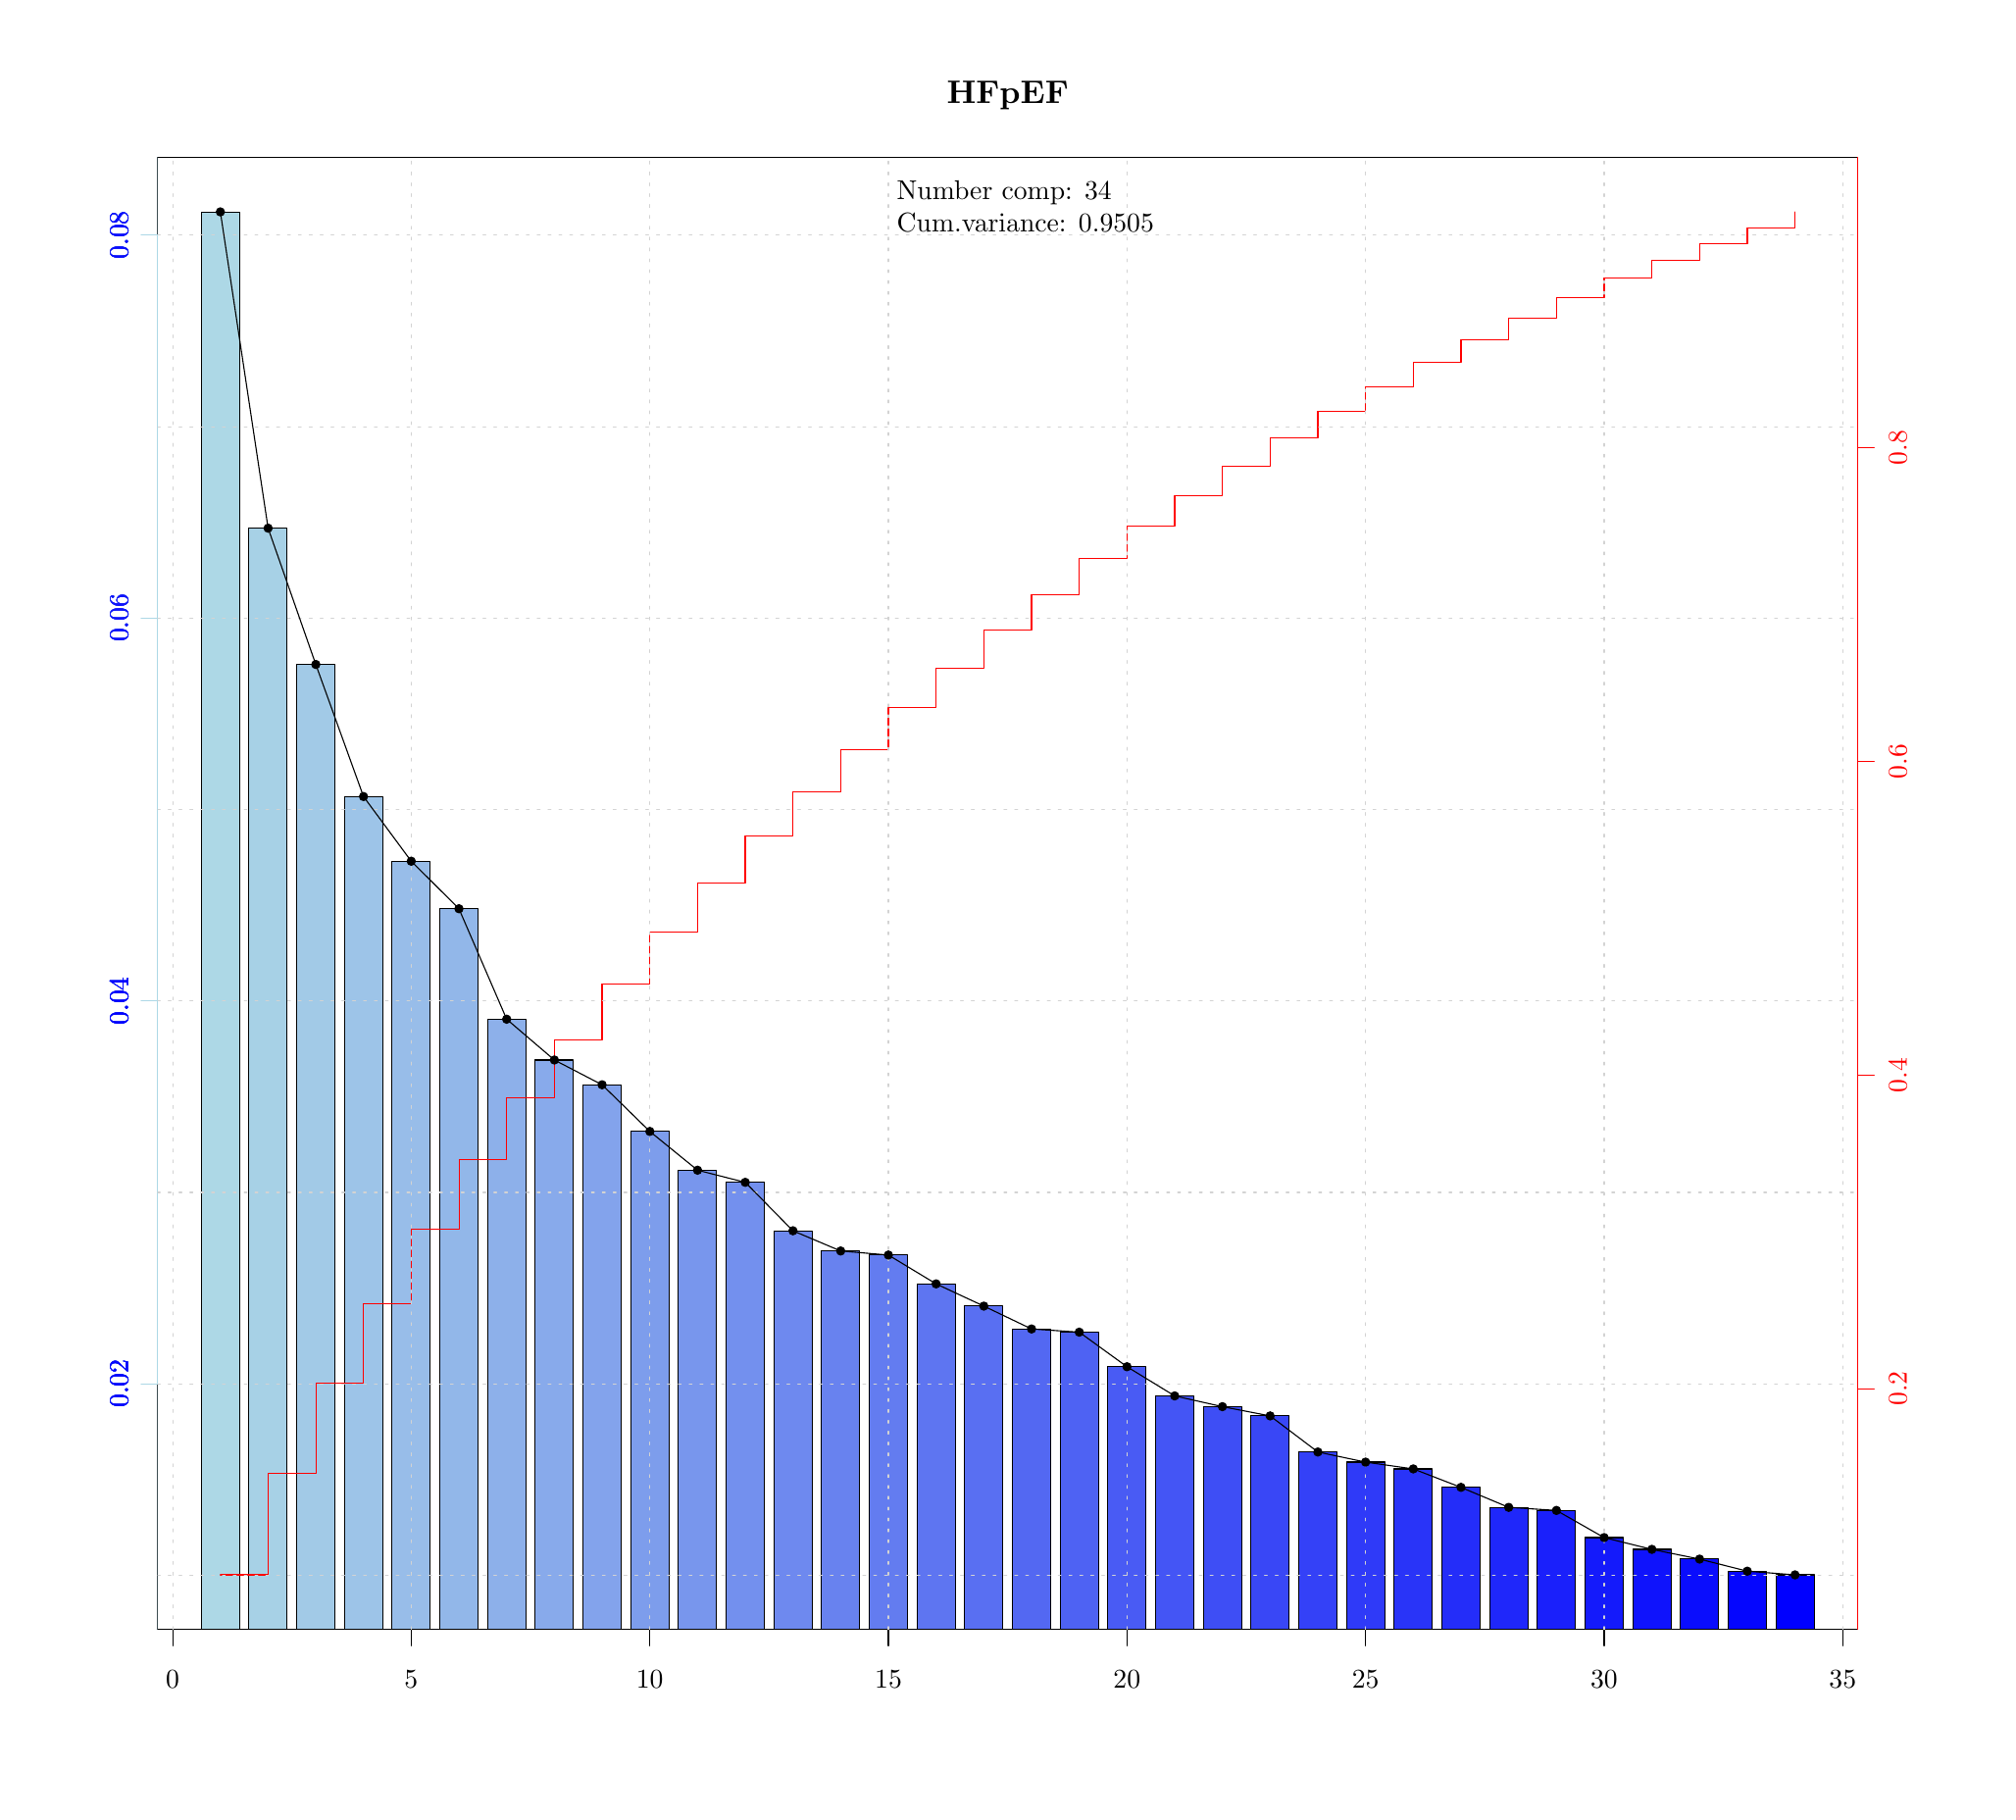
\begin{tikzpicture}[x=1pt,y=1pt]
\definecolor{fillColor}{RGB}{255,255,255}
\path[use as bounding box,fill=fillColor,fill opacity=0.00] (0,0) rectangle (722.70,650.43);
\begin{scope}
\path[clip] ( 48.00, 60.00) rectangle (674.70,602.43);
\definecolor{drawColor}{RGB}{0,0,0}
\definecolor{fillColor}{RGB}{173,216,230}

\path[draw=drawColor,line width= 0.4pt,line join=round,line cap=round,fill=fillColor] ( 64.18, 60.00) rectangle ( 78.24,582.34);
\definecolor{fillColor}{RGB}{167,209,230}

\path[draw=drawColor,line width= 0.4pt,line join=round,line cap=round,fill=fillColor] ( 81.76, 60.00) rectangle ( 95.83,465.79);
\definecolor{fillColor}{RGB}{162,202,231}

\path[draw=drawColor,line width= 0.4pt,line join=round,line cap=round,fill=fillColor] ( 99.35, 60.00) rectangle (113.41,415.57);
\definecolor{fillColor}{RGB}{157,196,232}

\path[draw=drawColor,line width= 0.4pt,line join=round,line cap=round,fill=fillColor] (116.93, 60.00) rectangle (131.00,366.90);
\definecolor{fillColor}{RGB}{152,189,233}

\path[draw=drawColor,line width= 0.4pt,line join=round,line cap=round,fill=fillColor] (134.51, 60.00) rectangle (148.58,343.07);
\definecolor{fillColor}{RGB}{146,183,233}

\path[draw=drawColor,line width= 0.4pt,line join=round,line cap=round,fill=fillColor] (152.10, 60.00) rectangle (166.17,325.56);
\definecolor{fillColor}{RGB}{141,176,234}

\path[draw=drawColor,line width= 0.4pt,line join=round,line cap=round,fill=fillColor] (169.68, 60.00) rectangle (183.75,284.85);
\definecolor{fillColor}{RGB}{136,170,235}

\path[draw=drawColor,line width= 0.4pt,line join=round,line cap=round,fill=fillColor] (187.27, 60.00) rectangle (201.33,269.82);
\definecolor{fillColor}{RGB}{131,163,236}

\path[draw=drawColor,line width= 0.4pt,line join=round,line cap=round,fill=fillColor] (204.85, 60.00) rectangle (218.92,260.69);
\definecolor{fillColor}{RGB}{125,157,236}

\path[draw=drawColor,line width= 0.4pt,line join=round,line cap=round,fill=fillColor] (222.44, 60.00) rectangle (236.50,243.50);
\definecolor{fillColor}{RGB}{120,150,237}

\path[draw=drawColor,line width= 0.4pt,line join=round,line cap=round,fill=fillColor] (240.02, 60.00) rectangle (254.09,229.21);
\definecolor{fillColor}{RGB}{115,144,238}

\path[draw=drawColor,line width= 0.4pt,line join=round,line cap=round,fill=fillColor] (257.60, 60.00) rectangle (271.67,224.74);
\definecolor{fillColor}{RGB}{110,137,239}

\path[draw=drawColor,line width= 0.4pt,line join=round,line cap=round,fill=fillColor] (275.19, 60.00) rectangle (289.25,206.89);
\definecolor{fillColor}{RGB}{104,130,239}

\path[draw=drawColor,line width= 0.4pt,line join=round,line cap=round,fill=fillColor] (292.77, 60.00) rectangle (306.84,199.44);
\definecolor{fillColor}{RGB}{99,124,240}

\path[draw=drawColor,line width= 0.4pt,line join=round,line cap=round,fill=fillColor] (310.36, 60.00) rectangle (324.42,197.95);
\definecolor{fillColor}{RGB}{94,117,241}

\path[draw=drawColor,line width= 0.4pt,line join=round,line cap=round,fill=fillColor] (327.94, 60.00) rectangle (342.01,187.32);
\definecolor{fillColor}{RGB}{89,111,242}

\path[draw=drawColor,line width= 0.4pt,line join=round,line cap=round,fill=fillColor] (345.52, 60.00) rectangle (359.59,179.13);
\definecolor{fillColor}{RGB}{83,104,242}

\path[draw=drawColor,line width= 0.4pt,line join=round,line cap=round,fill=fillColor] (363.11, 60.00) rectangle (377.18,170.71);
\definecolor{fillColor}{RGB}{78,98,243}

\path[draw=drawColor,line width= 0.4pt,line join=round,line cap=round,fill=fillColor] (380.69, 60.00) rectangle (394.76,169.53);
\definecolor{fillColor}{RGB}{73,91,244}

\path[draw=drawColor,line width= 0.4pt,line join=round,line cap=round,fill=fillColor] (398.28, 60.00) rectangle (412.34,156.79);
\definecolor{fillColor}{RGB}{68,85,245}

\path[draw=drawColor,line width= 0.4pt,line join=round,line cap=round,fill=fillColor] (415.86, 60.00) rectangle (429.93,146.04);
\definecolor{fillColor}{RGB}{62,78,245}

\path[draw=drawColor,line width= 0.4pt,line join=round,line cap=round,fill=fillColor] (433.45, 60.00) rectangle (447.51,142.08);
\definecolor{fillColor}{RGB}{57,71,246}

\path[draw=drawColor,line width= 0.4pt,line join=round,line cap=round,fill=fillColor] (451.03, 60.00) rectangle (465.10,138.67);
\definecolor{fillColor}{RGB}{52,65,247}

\path[draw=drawColor,line width= 0.4pt,line join=round,line cap=round,fill=fillColor] (468.61, 60.00) rectangle (482.68,125.37);
\definecolor{fillColor}{RGB}{47,58,248}

\path[draw=drawColor,line width= 0.4pt,line join=round,line cap=round,fill=fillColor] (486.20, 60.00) rectangle (500.26,121.64);
\definecolor{fillColor}{RGB}{41,52,248}

\path[draw=drawColor,line width= 0.4pt,line join=round,line cap=round,fill=fillColor] (503.78, 60.00) rectangle (517.85,119.14);
\definecolor{fillColor}{RGB}{36,45,249}

\path[draw=drawColor,line width= 0.4pt,line join=round,line cap=round,fill=fillColor] (521.37, 60.00) rectangle (535.43,112.34);
\definecolor{fillColor}{RGB}{31,39,250}

\path[draw=drawColor,line width= 0.4pt,line join=round,line cap=round,fill=fillColor] (538.95, 60.00) rectangle (553.02,104.97);
\definecolor{fillColor}{RGB}{26,32,251}

\path[draw=drawColor,line width= 0.4pt,line join=round,line cap=round,fill=fillColor] (556.53, 60.00) rectangle (570.60,103.84);
\definecolor{fillColor}{RGB}{20,26,251}

\path[draw=drawColor,line width= 0.4pt,line join=round,line cap=round,fill=fillColor] (574.12, 60.00) rectangle (588.19, 93.83);
\definecolor{fillColor}{RGB}{15,19,252}

\path[draw=drawColor,line width= 0.4pt,line join=round,line cap=round,fill=fillColor] (591.70, 60.00) rectangle (605.77, 89.49);
\definecolor{fillColor}{RGB}{10,13,253}

\path[draw=drawColor,line width= 0.4pt,line join=round,line cap=round,fill=fillColor] (609.29, 60.00) rectangle (623.35, 85.91);
\definecolor{fillColor}{RGB}{5,6,254}

\path[draw=drawColor,line width= 0.4pt,line join=round,line cap=round,fill=fillColor] (626.87, 60.00) rectangle (640.94, 81.45);
\definecolor{fillColor}{RGB}{0,0,255}

\path[draw=drawColor,line width= 0.4pt,line join=round,line cap=round,fill=fillColor] (644.46, 60.00) rectangle (658.52, 80.09);
\end{scope}
\begin{scope}
\path[clip] (  0.00,  0.00) rectangle (722.70,650.43);
\definecolor{drawColor}{RGB}{0,0,0}

\node[text=drawColor,anchor=base,inner sep=0pt, outer sep=0pt, scale=  1.20] at (361.35,622.29) {\bfseries HFpEF};
\end{scope}
\begin{scope}
\path[clip] (  0.00,  0.00) rectangle (722.70,650.43);
\definecolor{drawColor}{RGB}{0,0,0}

\path[draw=drawColor,line width= 0.4pt,line join=round,line cap=round] ( 48.00, 60.00) --
	(674.70, 60.00) --
	(674.70,602.43) --
	( 48.00,602.43) --
	( 48.00, 60.00);

\path[draw=drawColor,line width= 0.4pt,line join=round,line cap=round] ( 53.63, 60.00) -- (669.07, 60.00);

\path[draw=drawColor,line width= 0.4pt,line join=round,line cap=round] ( 53.63, 60.00) -- ( 53.63, 54.00);

\path[draw=drawColor,line width= 0.4pt,line join=round,line cap=round] (141.55, 60.00) -- (141.55, 54.00);

\path[draw=drawColor,line width= 0.4pt,line join=round,line cap=round] (229.47, 60.00) -- (229.47, 54.00);

\path[draw=drawColor,line width= 0.4pt,line join=round,line cap=round] (317.39, 60.00) -- (317.39, 54.00);

\path[draw=drawColor,line width= 0.4pt,line join=round,line cap=round] (405.31, 60.00) -- (405.31, 54.00);

\path[draw=drawColor,line width= 0.4pt,line join=round,line cap=round] (493.23, 60.00) -- (493.23, 54.00);

\path[draw=drawColor,line width= 0.4pt,line join=round,line cap=round] (581.15, 60.00) -- (581.15, 54.00);

\path[draw=drawColor,line width= 0.4pt,line join=round,line cap=round] (669.07, 60.00) -- (669.07, 54.00);

\node[text=drawColor,anchor=base,inner sep=0pt, outer sep=0pt, scale=  1.00] at ( 53.63, 38.40) {0};

\node[text=drawColor,anchor=base,inner sep=0pt, outer sep=0pt, scale=  1.00] at (141.55, 38.40) {5};

\node[text=drawColor,anchor=base,inner sep=0pt, outer sep=0pt, scale=  1.00] at (229.47, 38.40) {10};

\node[text=drawColor,anchor=base,inner sep=0pt, outer sep=0pt, scale=  1.00] at (317.39, 38.40) {15};

\node[text=drawColor,anchor=base,inner sep=0pt, outer sep=0pt, scale=  1.00] at (405.31, 38.40) {20};

\node[text=drawColor,anchor=base,inner sep=0pt, outer sep=0pt, scale=  1.00] at (493.23, 38.40) {25};

\node[text=drawColor,anchor=base,inner sep=0pt, outer sep=0pt, scale=  1.00] at (581.15, 38.40) {30};

\node[text=drawColor,anchor=base,inner sep=0pt, outer sep=0pt, scale=  1.00] at (669.07, 38.40) {35};
\definecolor{drawColor}{RGB}{173,216,230}

\path[draw=drawColor,line width= 0.4pt,line join=round,line cap=round] ( 48.00,150.48) -- ( 48.00,573.75);

\path[draw=drawColor,line width= 0.4pt,line join=round,line cap=round] ( 48.00,150.48) -- ( 42.00,150.48);

\path[draw=drawColor,line width= 0.4pt,line join=round,line cap=round] ( 48.00,291.57) -- ( 42.00,291.57);

\path[draw=drawColor,line width= 0.4pt,line join=round,line cap=round] ( 48.00,432.66) -- ( 42.00,432.66);

\path[draw=drawColor,line width= 0.4pt,line join=round,line cap=round] ( 48.00,573.75) -- ( 42.00,573.75);

\node[text=drawColor,rotate= 90.00,anchor=base,inner sep=0pt, outer sep=0pt, scale=  1.00] at ( 37.20,150.48) {0.02};
\definecolor{drawColor}{RGB}{167,209,230}

\node[text=drawColor,rotate= 90.00,anchor=base,inner sep=0pt, outer sep=0pt, scale=  1.00] at ( 37.20,291.57) {0.04};
\definecolor{drawColor}{RGB}{162,202,231}

\node[text=drawColor,rotate= 90.00,anchor=base,inner sep=0pt, outer sep=0pt, scale=  1.00] at ( 37.20,432.66) {0.06};
\definecolor{drawColor}{RGB}{157,196,232}

\node[text=drawColor,rotate= 90.00,anchor=base,inner sep=0pt, outer sep=0pt, scale=  1.00] at ( 37.20,573.75) {0.08};
\definecolor{drawColor}{RGB}{152,189,233}

\node[text=drawColor,rotate= 90.00,anchor=base,inner sep=0pt, outer sep=0pt, scale=  1.00] at ( 37.20,150.48) {0.02};
\definecolor{drawColor}{RGB}{146,183,233}

\node[text=drawColor,rotate= 90.00,anchor=base,inner sep=0pt, outer sep=0pt, scale=  1.00] at ( 37.20,291.57) {0.04};
\definecolor{drawColor}{RGB}{141,176,234}

\node[text=drawColor,rotate= 90.00,anchor=base,inner sep=0pt, outer sep=0pt, scale=  1.00] at ( 37.20,432.66) {0.06};
\definecolor{drawColor}{RGB}{136,170,235}

\node[text=drawColor,rotate= 90.00,anchor=base,inner sep=0pt, outer sep=0pt, scale=  1.00] at ( 37.20,573.75) {0.08};
\definecolor{drawColor}{RGB}{131,163,236}

\node[text=drawColor,rotate= 90.00,anchor=base,inner sep=0pt, outer sep=0pt, scale=  1.00] at ( 37.20,150.48) {0.02};
\definecolor{drawColor}{RGB}{125,157,236}

\node[text=drawColor,rotate= 90.00,anchor=base,inner sep=0pt, outer sep=0pt, scale=  1.00] at ( 37.20,291.57) {0.04};
\definecolor{drawColor}{RGB}{120,150,237}

\node[text=drawColor,rotate= 90.00,anchor=base,inner sep=0pt, outer sep=0pt, scale=  1.00] at ( 37.20,432.66) {0.06};
\definecolor{drawColor}{RGB}{115,144,238}

\node[text=drawColor,rotate= 90.00,anchor=base,inner sep=0pt, outer sep=0pt, scale=  1.00] at ( 37.20,573.75) {0.08};
\definecolor{drawColor}{RGB}{110,137,239}

\node[text=drawColor,rotate= 90.00,anchor=base,inner sep=0pt, outer sep=0pt, scale=  1.00] at ( 37.20,150.48) {0.02};
\definecolor{drawColor}{RGB}{104,130,239}

\node[text=drawColor,rotate= 90.00,anchor=base,inner sep=0pt, outer sep=0pt, scale=  1.00] at ( 37.20,291.57) {0.04};
\definecolor{drawColor}{RGB}{99,124,240}

\node[text=drawColor,rotate= 90.00,anchor=base,inner sep=0pt, outer sep=0pt, scale=  1.00] at ( 37.20,432.66) {0.06};
\definecolor{drawColor}{RGB}{94,117,241}

\node[text=drawColor,rotate= 90.00,anchor=base,inner sep=0pt, outer sep=0pt, scale=  1.00] at ( 37.20,573.75) {0.08};
\definecolor{drawColor}{RGB}{89,111,242}

\node[text=drawColor,rotate= 90.00,anchor=base,inner sep=0pt, outer sep=0pt, scale=  1.00] at ( 37.20,150.48) {0.02};
\definecolor{drawColor}{RGB}{83,104,242}

\node[text=drawColor,rotate= 90.00,anchor=base,inner sep=0pt, outer sep=0pt, scale=  1.00] at ( 37.20,291.57) {0.04};
\definecolor{drawColor}{RGB}{78,98,243}

\node[text=drawColor,rotate= 90.00,anchor=base,inner sep=0pt, outer sep=0pt, scale=  1.00] at ( 37.20,432.66) {0.06};
\definecolor{drawColor}{RGB}{73,91,244}

\node[text=drawColor,rotate= 90.00,anchor=base,inner sep=0pt, outer sep=0pt, scale=  1.00] at ( 37.20,573.75) {0.08};
\definecolor{drawColor}{RGB}{68,85,245}

\node[text=drawColor,rotate= 90.00,anchor=base,inner sep=0pt, outer sep=0pt, scale=  1.00] at ( 37.20,150.48) {0.02};
\definecolor{drawColor}{RGB}{62,78,245}

\node[text=drawColor,rotate= 90.00,anchor=base,inner sep=0pt, outer sep=0pt, scale=  1.00] at ( 37.20,291.57) {0.04};
\definecolor{drawColor}{RGB}{57,71,246}

\node[text=drawColor,rotate= 90.00,anchor=base,inner sep=0pt, outer sep=0pt, scale=  1.00] at ( 37.20,432.66) {0.06};
\definecolor{drawColor}{RGB}{52,65,247}

\node[text=drawColor,rotate= 90.00,anchor=base,inner sep=0pt, outer sep=0pt, scale=  1.00] at ( 37.20,573.75) {0.08};
\definecolor{drawColor}{RGB}{47,58,248}

\node[text=drawColor,rotate= 90.00,anchor=base,inner sep=0pt, outer sep=0pt, scale=  1.00] at ( 37.20,150.48) {0.02};
\definecolor{drawColor}{RGB}{41,52,248}

\node[text=drawColor,rotate= 90.00,anchor=base,inner sep=0pt, outer sep=0pt, scale=  1.00] at ( 37.20,291.57) {0.04};
\definecolor{drawColor}{RGB}{36,45,249}

\node[text=drawColor,rotate= 90.00,anchor=base,inner sep=0pt, outer sep=0pt, scale=  1.00] at ( 37.20,432.66) {0.06};
\definecolor{drawColor}{RGB}{31,39,250}

\node[text=drawColor,rotate= 90.00,anchor=base,inner sep=0pt, outer sep=0pt, scale=  1.00] at ( 37.20,573.75) {0.08};
\definecolor{drawColor}{RGB}{26,32,251}

\node[text=drawColor,rotate= 90.00,anchor=base,inner sep=0pt, outer sep=0pt, scale=  1.00] at ( 37.20,150.48) {0.02};
\definecolor{drawColor}{RGB}{20,26,251}

\node[text=drawColor,rotate= 90.00,anchor=base,inner sep=0pt, outer sep=0pt, scale=  1.00] at ( 37.20,291.57) {0.04};
\definecolor{drawColor}{RGB}{15,19,252}

\node[text=drawColor,rotate= 90.00,anchor=base,inner sep=0pt, outer sep=0pt, scale=  1.00] at ( 37.20,432.66) {0.06};
\definecolor{drawColor}{RGB}{10,13,253}

\node[text=drawColor,rotate= 90.00,anchor=base,inner sep=0pt, outer sep=0pt, scale=  1.00] at ( 37.20,573.75) {0.08};
\definecolor{drawColor}{RGB}{5,6,254}

\node[text=drawColor,rotate= 90.00,anchor=base,inner sep=0pt, outer sep=0pt, scale=  1.00] at ( 37.20,150.48) {0.02};
\definecolor{drawColor}{RGB}{0,0,255}

\node[text=drawColor,rotate= 90.00,anchor=base,inner sep=0pt, outer sep=0pt, scale=  1.00] at ( 37.20,291.57) {0.04};
\end{scope}
\begin{scope}
\path[clip] ( 48.00, 60.00) rectangle (674.70,602.43);
\definecolor{drawColor}{RGB}{173,216,230}

\path[draw=drawColor,line width= 0.4pt,line join=round,line cap=round] ( 48.00, 60.00) -- ( 48.00,602.43);
\definecolor{drawColor}{RGB}{255,0,0}

\path[draw=drawColor,line width= 0.4pt,line join=round,line cap=round] ( 71.21, 80.09) --
	( 88.80, 80.09) --
	( 88.80,117.47) --
	(106.38,117.47) --
	(106.38,150.74) --
	(123.96,150.74) --
	(123.96,180.02) --
	(141.55,180.02) --
	(141.55,207.34) --
	(159.13,207.34) --
	(159.13,233.24) --
	(176.72,233.24) --
	(176.72,255.80) --
	(194.30,255.80) --
	(194.30,277.13) --
	(211.88,277.13) --
	(211.88,297.71) --
	(229.47,297.71) --
	(229.47,316.88) --
	(247.05,316.88) --
	(247.05,334.89) --
	(264.64,334.89) --
	(264.64,352.52) --
	(282.22,352.52) --
	(282.22,368.70) --
	(299.81,368.70) --
	(299.81,384.26) --
	(317.39,384.26) --
	(317.39,399.71) --
	(334.97,399.71) --
	(334.97,414.28) --
	(352.56,414.28) --
	(352.56,428.18) --
	(370.14,428.18) --
	(370.14,441.39) --
	(387.73,441.39) --
	(387.73,454.51) --
	(405.31,454.51) --
	(405.31,466.58) --
	(422.89,466.58) --
	(422.89,477.77) --
	(440.48,477.77) --
	(440.48,488.64) --
	(458.06,488.64) --
	(458.06,499.23) --
	(475.65,499.23) --
	(475.65,508.73) --
	(493.23,508.73) --
	(493.23,517.92) --
	(510.82,517.92) --
	(510.82,526.91) --
	(528.40,526.91) --
	(528.40,535.34) --
	(545.98,535.34) --
	(545.98,543.17) --
	(563.57,543.17) --
	(563.57,550.90) --
	(581.15,550.90) --
	(581.15,557.82) --
	(598.74,557.82) --
	(598.74,564.38) --
	(616.32,564.38) --
	(616.32,570.65) --
	(633.90,570.65) --
	(633.90,576.55) --
	(651.49,576.55) --
	(651.49,582.34);
\end{scope}
\begin{scope}
\path[clip] (  0.00,  0.00) rectangle (722.70,650.43);
\definecolor{drawColor}{RGB}{255,0,0}

\path[draw=drawColor,line width= 0.4pt,line join=round,line cap=round] (674.70,148.72) -- (674.70,495.37);

\path[draw=drawColor,line width= 0.4pt,line join=round,line cap=round] (674.70,148.72) -- (680.70,148.72);

\path[draw=drawColor,line width= 0.4pt,line join=round,line cap=round] (674.70,264.27) -- (680.70,264.27);

\path[draw=drawColor,line width= 0.4pt,line join=round,line cap=round] (674.70,379.82) -- (680.70,379.82);

\path[draw=drawColor,line width= 0.4pt,line join=round,line cap=round] (674.70,495.37) -- (680.70,495.37);

\node[text=drawColor,rotate= 90.00,anchor=base,inner sep=0pt, outer sep=0pt, scale=  1.00] at (692.70,148.72) {0.2};

\node[text=drawColor,rotate= 90.00,anchor=base,inner sep=0pt, outer sep=0pt, scale=  1.00] at (692.70,264.27) {0.4};

\node[text=drawColor,rotate= 90.00,anchor=base,inner sep=0pt, outer sep=0pt, scale=  1.00] at (692.70,379.82) {0.6};

\node[text=drawColor,rotate= 90.00,anchor=base,inner sep=0pt, outer sep=0pt, scale=  1.00] at (692.70,495.37) {0.8};
\end{scope}
\begin{scope}
\path[clip] ( 48.00, 60.00) rectangle (674.70,602.43);
\definecolor{drawColor}{RGB}{255,0,0}

\path[draw=drawColor,line width= 0.4pt,line join=round,line cap=round] (674.70, 60.00) -- (674.70,602.43);
\definecolor{drawColor}{RGB}{211,211,211}

\path[draw=drawColor,line width= 0.4pt,dash pattern=on 1pt off 3pt ,line join=round,line cap=round] ( 53.63, 60.00) -- ( 53.63,602.43);

\path[draw=drawColor,line width= 0.4pt,dash pattern=on 1pt off 3pt ,line join=round,line cap=round] (141.55, 60.00) -- (141.55,602.43);

\path[draw=drawColor,line width= 0.4pt,dash pattern=on 1pt off 3pt ,line join=round,line cap=round] (229.47, 60.00) -- (229.47,602.43);

\path[draw=drawColor,line width= 0.4pt,dash pattern=on 1pt off 3pt ,line join=round,line cap=round] (317.39, 60.00) -- (317.39,602.43);

\path[draw=drawColor,line width= 0.4pt,dash pattern=on 1pt off 3pt ,line join=round,line cap=round] (405.31, 60.00) -- (405.31,602.43);

\path[draw=drawColor,line width= 0.4pt,dash pattern=on 1pt off 3pt ,line join=round,line cap=round] (493.23, 60.00) -- (493.23,602.43);

\path[draw=drawColor,line width= 0.4pt,dash pattern=on 1pt off 3pt ,line join=round,line cap=round] (581.15, 60.00) -- (581.15,602.43);

\path[draw=drawColor,line width= 0.4pt,dash pattern=on 1pt off 3pt ,line join=round,line cap=round] (669.07, 60.00) -- (669.07,602.43);

\path[draw=drawColor,line width= 0.4pt,dash pattern=on 1pt off 3pt ,line join=round,line cap=round] ( 48.00, 79.93) -- (674.70, 79.93);

\path[draw=drawColor,line width= 0.4pt,dash pattern=on 1pt off 3pt ,line join=round,line cap=round] ( 48.00,150.48) -- (674.70,150.48);

\path[draw=drawColor,line width= 0.4pt,dash pattern=on 1pt off 3pt ,line join=round,line cap=round] ( 48.00,221.02) -- (674.70,221.02);

\path[draw=drawColor,line width= 0.4pt,dash pattern=on 1pt off 3pt ,line join=round,line cap=round] ( 48.00,291.57) -- (674.70,291.57);

\path[draw=drawColor,line width= 0.4pt,dash pattern=on 1pt off 3pt ,line join=round,line cap=round] ( 48.00,362.11) -- (674.70,362.11);

\path[draw=drawColor,line width= 0.4pt,dash pattern=on 1pt off 3pt ,line join=round,line cap=round] ( 48.00,432.66) -- (674.70,432.66);

\path[draw=drawColor,line width= 0.4pt,dash pattern=on 1pt off 3pt ,line join=round,line cap=round] ( 48.00,503.20) -- (674.70,503.20);

\path[draw=drawColor,line width= 0.4pt,dash pattern=on 1pt off 3pt ,line join=round,line cap=round] ( 48.00,573.75) -- (674.70,573.75);
\definecolor{drawColor}{RGB}{0,0,0}

\path[draw=drawColor,line width= 0.4pt,line join=round,line cap=round] ( 71.21,582.34) --
	( 88.80,465.79) --
	(106.38,415.57) --
	(123.96,366.90) --
	(141.55,343.07) --
	(159.13,325.56) --
	(176.72,284.85) --
	(194.30,269.82) --
	(211.88,260.69) --
	(229.47,243.50) --
	(247.05,229.21) --
	(264.64,224.74) --
	(282.22,206.89) --
	(299.81,199.44) --
	(317.39,197.95) --
	(334.97,187.32) --
	(352.56,179.13) --
	(370.14,170.71) --
	(387.73,169.53) --
	(405.31,156.79) --
	(422.89,146.04) --
	(440.48,142.08) --
	(458.06,138.67) --
	(475.65,125.37) --
	(493.23,121.64) --
	(510.82,119.14) --
	(528.40,112.34) --
	(545.98,104.97) --
	(563.57,103.84) --
	(581.15, 93.83) --
	(598.74, 89.49) --
	(616.32, 85.91) --
	(633.90, 81.45) --
	(651.49, 80.09);
\definecolor{fillColor}{RGB}{0,0,0}

\path[draw=drawColor,line width= 0.4pt,line join=round,line cap=round,fill=fillColor] ( 71.21,582.34) circle (  1.50);

\path[draw=drawColor,line width= 0.4pt,line join=round,line cap=round,fill=fillColor] ( 88.80,465.79) circle (  1.50);

\path[draw=drawColor,line width= 0.4pt,line join=round,line cap=round,fill=fillColor] (106.38,415.57) circle (  1.50);

\path[draw=drawColor,line width= 0.4pt,line join=round,line cap=round,fill=fillColor] (123.96,366.90) circle (  1.50);

\path[draw=drawColor,line width= 0.4pt,line join=round,line cap=round,fill=fillColor] (141.55,343.07) circle (  1.50);

\path[draw=drawColor,line width= 0.4pt,line join=round,line cap=round,fill=fillColor] (159.13,325.56) circle (  1.50);

\path[draw=drawColor,line width= 0.4pt,line join=round,line cap=round,fill=fillColor] (176.72,284.85) circle (  1.50);

\path[draw=drawColor,line width= 0.4pt,line join=round,line cap=round,fill=fillColor] (194.30,269.82) circle (  1.50);

\path[draw=drawColor,line width= 0.4pt,line join=round,line cap=round,fill=fillColor] (211.88,260.69) circle (  1.50);

\path[draw=drawColor,line width= 0.4pt,line join=round,line cap=round,fill=fillColor] (229.47,243.50) circle (  1.50);

\path[draw=drawColor,line width= 0.4pt,line join=round,line cap=round,fill=fillColor] (247.05,229.21) circle (  1.50);

\path[draw=drawColor,line width= 0.4pt,line join=round,line cap=round,fill=fillColor] (264.64,224.74) circle (  1.50);

\path[draw=drawColor,line width= 0.4pt,line join=round,line cap=round,fill=fillColor] (282.22,206.89) circle (  1.50);

\path[draw=drawColor,line width= 0.4pt,line join=round,line cap=round,fill=fillColor] (299.81,199.44) circle (  1.50);

\path[draw=drawColor,line width= 0.4pt,line join=round,line cap=round,fill=fillColor] (317.39,197.95) circle (  1.50);

\path[draw=drawColor,line width= 0.4pt,line join=round,line cap=round,fill=fillColor] (334.97,187.32) circle (  1.50);

\path[draw=drawColor,line width= 0.4pt,line join=round,line cap=round,fill=fillColor] (352.56,179.13) circle (  1.50);

\path[draw=drawColor,line width= 0.4pt,line join=round,line cap=round,fill=fillColor] (370.14,170.71) circle (  1.50);

\path[draw=drawColor,line width= 0.4pt,line join=round,line cap=round,fill=fillColor] (387.73,169.53) circle (  1.50);

\path[draw=drawColor,line width= 0.4pt,line join=round,line cap=round,fill=fillColor] (405.31,156.79) circle (  1.50);

\path[draw=drawColor,line width= 0.4pt,line join=round,line cap=round,fill=fillColor] (422.89,146.04) circle (  1.50);

\path[draw=drawColor,line width= 0.4pt,line join=round,line cap=round,fill=fillColor] (440.48,142.08) circle (  1.50);

\path[draw=drawColor,line width= 0.4pt,line join=round,line cap=round,fill=fillColor] (458.06,138.67) circle (  1.50);

\path[draw=drawColor,line width= 0.4pt,line join=round,line cap=round,fill=fillColor] (475.65,125.37) circle (  1.50);

\path[draw=drawColor,line width= 0.4pt,line join=round,line cap=round,fill=fillColor] (493.23,121.64) circle (  1.50);

\path[draw=drawColor,line width= 0.4pt,line join=round,line cap=round,fill=fillColor] (510.82,119.14) circle (  1.50);

\path[draw=drawColor,line width= 0.4pt,line join=round,line cap=round,fill=fillColor] (528.40,112.34) circle (  1.50);

\path[draw=drawColor,line width= 0.4pt,line join=round,line cap=round,fill=fillColor] (545.98,104.97) circle (  1.50);

\path[draw=drawColor,line width= 0.4pt,line join=round,line cap=round,fill=fillColor] (563.57,103.84) circle (  1.50);

\path[draw=drawColor,line width= 0.4pt,line join=round,line cap=round,fill=fillColor] (581.15, 93.83) circle (  1.50);

\path[draw=drawColor,line width= 0.4pt,line join=round,line cap=round,fill=fillColor] (598.74, 89.49) circle (  1.50);

\path[draw=drawColor,line width= 0.4pt,line join=round,line cap=round,fill=fillColor] (616.32, 85.91) circle (  1.50);

\path[draw=drawColor,line width= 0.4pt,line join=round,line cap=round,fill=fillColor] (633.90, 81.45) circle (  1.50);

\path[draw=drawColor,line width= 0.4pt,line join=round,line cap=round,fill=fillColor] (651.49, 80.09) circle (  1.50);

\node[text=drawColor,anchor=base west,inner sep=0pt, outer sep=0pt, scale=  1.00] at (320.51,586.93) {Number comp: 34};

\node[text=drawColor,anchor=base west,inner sep=0pt, outer sep=0pt, scale=  1.00] at (320.51,574.88) {Cum.variance: 0.9505};
\end{scope}
\end{tikzpicture}
